\section{Explainability: Grad-CAM}
\label{sec:gradcam}

\paragraph{Implementation.}
We use Gradient-weighted Class Activation Mapping
(Grad-CAM~\cite{selvaraju2017gradcam}) to produce coarse spatial heatmaps
that highlight which image regions drive each prediction.
For the last convolutional layer producing feature maps
$A^k \in \mathbb{R}^{h \times w}$, the heatmap for target class $c$ is:
\begin{equation}
  L^c = \mathrm{ReLU}\!\Bigl(\sum_k \alpha_k^c\, A^k\Bigr),\quad
  \alpha_k^c = \frac{1}{Z}\sum_{i,j}
    \frac{\partial y^c}{\partial A^k_{ij}}
  \label{eq:gradcam}
\end{equation}
Hooks are attached to \texttt{layer4[-1].conv2} of the ResNet18 backbone
via \texttt{register\_forward\_hook} and
\texttt{register\_full\_backward\_hook}.
For the Hybrid model, the hook is placed on the RGB branch (spatial features
are more amenable to pixel-level interpretation).
The resulting heatmap is bilinearly upsampled to input resolution and blended
over the original image (weight\,=\,0.45) using a JET colour map.

\paragraph{Correct vs.\ failure cases.}
\cref{fig:gradcam} contrasts Grad-CAM heatmaps for correctly classified
faces (\cref{fig:gradcam_correct}) with the Hybrid model's failure cases
(\cref{fig:gradcam_fail}).
For correct predictions, attention concentrates on central face-internal
regions — the eyes, nose, and mouth — precisely where StyleGAN2's synthesis
is most complex and artefact-prone, indicating that the model has learned
semantically meaningful features rather than dataset-specific shortcuts.
The failure cases (real faces misclassified as fake) instead tend to exhibit
unusual lighting, heavy make-up, or extreme facial expressions — surface
characteristics the model associates with GAN-generated texture patterns.

\begin{figure*}[t]
  \centering
  \begin{subfigure}[t]{0.49\textwidth}
    \centering
    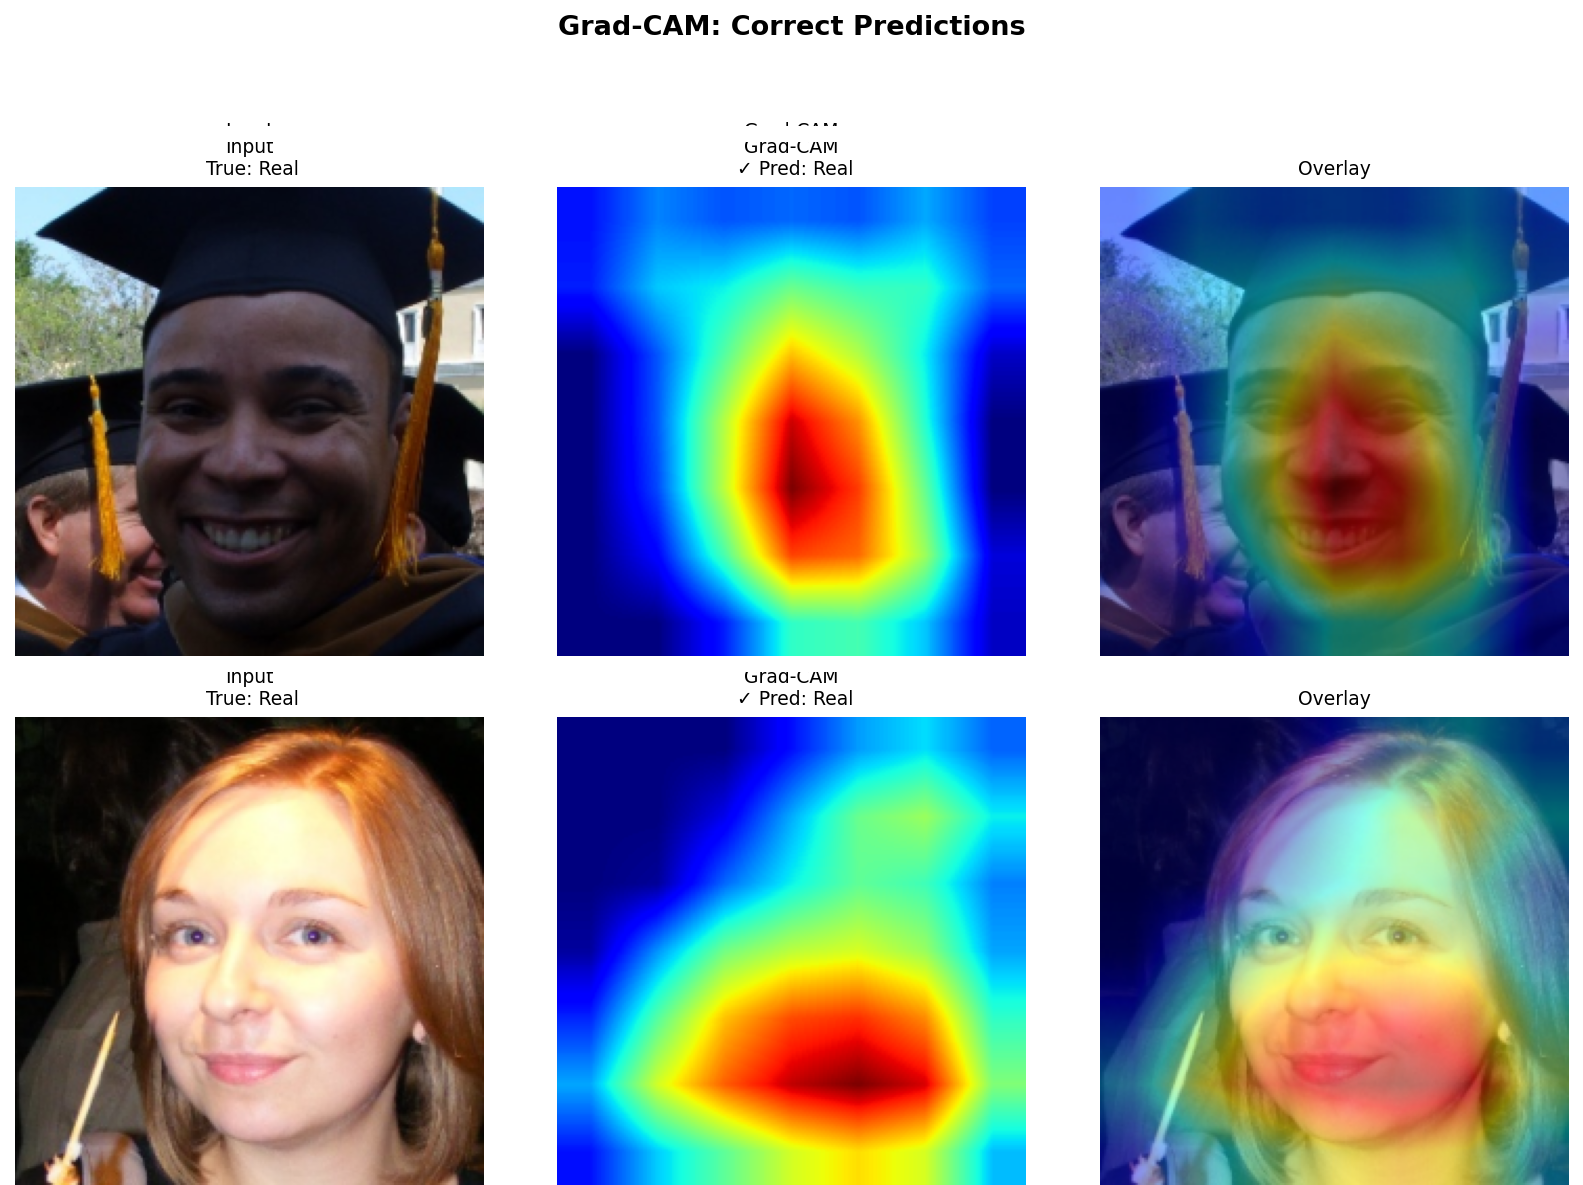
\includegraphics[width=\linewidth]{results/figures/gradcam_correct_pair.png}
    \caption{Correct predictions (real faces, correctly classified).}
    \label{fig:gradcam_correct}
  \end{subfigure}\hfill
  \begin{subfigure}[t]{0.49\textwidth}
    \centering
    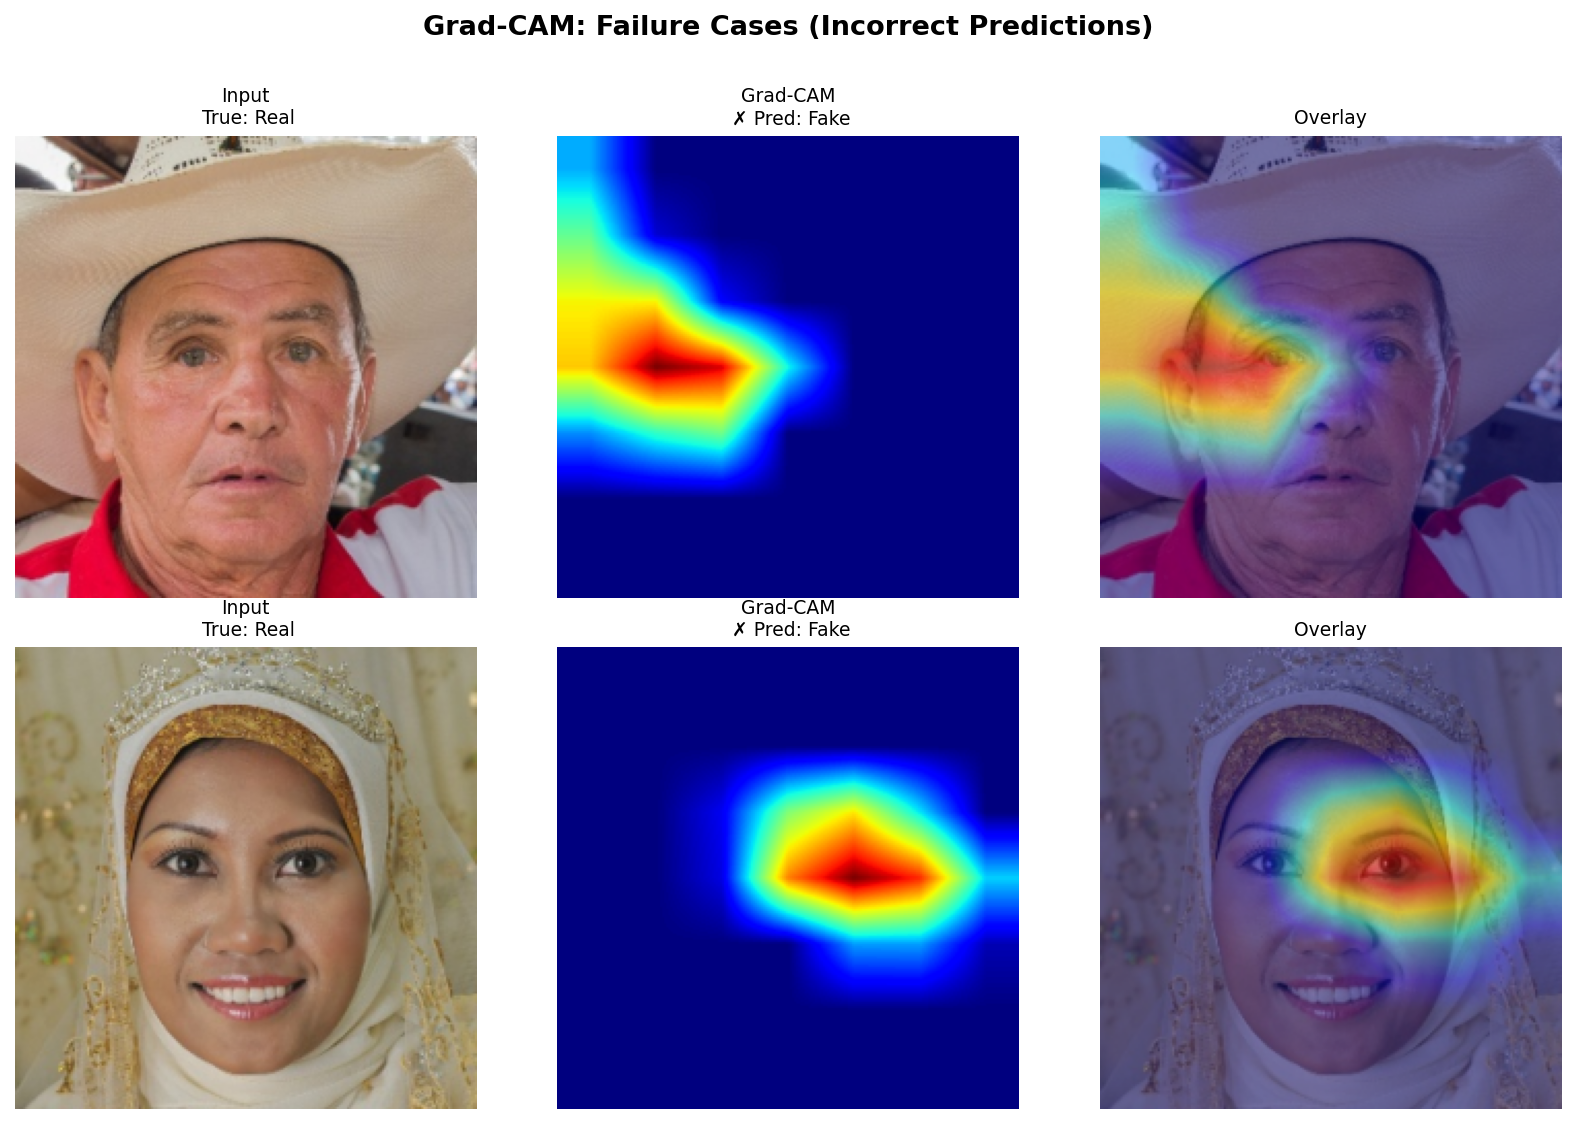
\includegraphics[width=\linewidth]{results/figures/gradcam_hybrid/gradcam_incorrect.png}
    \caption{Failure cases (real faces misclassified as fake).}
    \label{fig:gradcam_fail}
  \end{subfigure}
  \caption{%
    \textbf{Grad-CAM visualisations for the Hybrid model.}
    In every panel each row shows the input face (left), the Grad-CAM
    heatmap (middle), and the blended overlay (right).
    \textbf{(a)}~Correctly classified real faces — attention concentrates on
    central face-internal regions (eyes, nose, mouth).
    \textbf{(b)}~Misclassified real faces (predicted fake) — these cluster on
    images with unusual lighting, heavy cosmetics, or strong expression,
    surface patterns the model associates with GAN texture.
  }
  \label{fig:gradcam}
\end{figure*}
